\documentclass[12pt]{article}

\usepackage[margin=0.5in]{geometry}
\usepackage{amsmath, amssymb}

\usepackage{tikz}
\usepackage{pgfplots}
\pgfplotsset{compat=1.17}

\usepackage{hyperref}
\renewcommand{\arraystretch}{1.6}

\newcommand{\psetheader}[4]{%
  \noindent
  \begin{minipage}[t]{0.6\textwidth}
    #1\\
    #2\\
    #3
  \end{minipage}%
  \hfill
  \begin{minipage}[t]{0.35\textwidth}
    \raggedleft #4
  \end{minipage}

  \vspace{0.5\baselineskip}
  \hrule
  \vspace{1em}
}

\title{Kalkulus Diferensial - Diskusi Sesi 6}
\author{Anas Azhar \\ FST - Matematika - 056413438 \\ Universitas Terbuka}
\date{\today}


\begin{document}

\psetheader
  {\textit{Kalkulus Diferensial} - Diskusi Sesi 6}
  {Universitas Terbuka, FST - Matematika, 2025.1}
  {Anas Azhar (056413438)}
  {Minggu, 16 November 2025}

\section*{Soal}
Tentukan luas maksimum dari segi empat yang diarsir pada gambar di bawah ini,
yang berada di bawah kurva $y = 8 - x^2$. Segi empat memiliki lebar $p = 2x$ dan tinggi $l = y = 8 - x^2$.

\noindent \textbf{Gambar Kurva dan Persegi Panjang}

\begin{center}
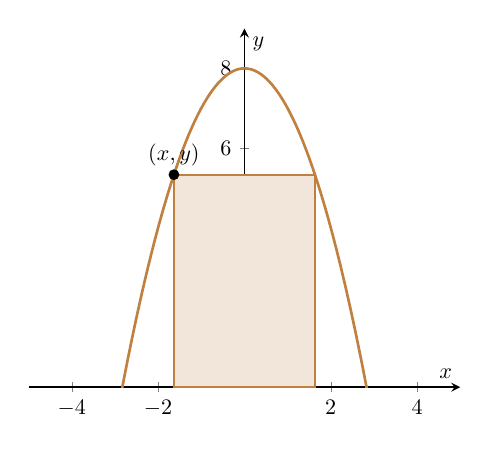
\begin{tikzpicture}[scale=0.8]
    \begin{axis}[
        axis lines=middle,
        xmin=-5, xmax=5,
        ymin=0, ymax=9,
        xlabel={$x$},
        ylabel={$y$},
        samples=200,
        domain=-3:3,
        thick
    ]
    % Kurva parabola
    \addplot[very thick, brown] {8 - x^2};

    % Persegi panjang: ambil x = sqrt(8/3)
    \pgfmathsetmacro{\xx}{sqrt(8/3)}
    \pgfmathsetmacro{\yy}{8 - (\xx)^2}

    % Persegi panjang
    \addplot[fill=brown!20, draw=brown]
        coordinates {(-\xx,0) (-\xx,\yy) (\xx,\yy) (\xx,0)} -- cycle;

    % Titik sudut kiri
    \addplot[black, only marks, mark=*] coordinates {(-\xx,\yy)};
    \node at (axis cs:-\xx,\yy+0.5) {$(x,y)$};
    \end{axis}
\end{tikzpicture}
\end{center}

\noindent \textbf{Penyelesaian}

\noindent Luas segi empat adalah
\[
A = \text{lebar} \times \text{tinggi}
= (2x)(8 - x^2).
\]

\noindent Maka fungsi luas:
\[
A(x) = 16x - 2x^3.
\]

\noindent Untuk mencari maksimum, turunkan:
\[
A'(x) = 16 - 6x^2.
\]

\noindent Set turunan = 0:
\[
16 - 6x^2 = 0
\quad \Rightarrow \quad
6x^2 = 16
\quad \Rightarrow \quad
x^2 = \frac{8}{3}
\quad \Rightarrow \quad
x = \sqrt{\frac{8}{3}}.
\]

\noindent Tinggi segi empat pada titik ini:
\[
y = 8 - x^2 = 8 - \frac{8}{3} = \frac{16}{3}.
\]

\noindent Maka luas maksimum:
\[
A_{\max}
= A\!\left(\sqrt{\frac{8}{3}}\right)
= 2x(8 - x^2)
= 2\sqrt{\frac{8}{3}}\left(\frac{16}{3}\right)
= \frac{32}{3}\sqrt{\frac{8}{3}}.
\]

\noindent Sederhanakan:
\[
\sqrt{\frac{8}{3}} = \frac{2\sqrt{6}}{3},
\]
maka
\[
A_{\max}
= \frac{32}{3} \cdot \frac{2\sqrt{6}}{3}
= \frac{64\sqrt{6}}{9}.
\]

\noindent \textbf{Jawaban Akhir}

\[
\boxed{
A_{\max} = \dfrac{64\sqrt{6}}{9} \text{Satuan Luas}
}
\]

\end{document}